%\Section{Dealing with crash failures}

In data-intensive applications, input data are divided into multiple splits that can be processed in parallel. To deal with crash failures, the Soft Replication computational model can be applied, with one fast replica and one slow replica assigned to each data split. The fast and slow replicas for the same split will process the split from two opposite ends, and complete the processing by meeting in some middle point, if no failure occurs. If one process fails, however, its associated process can continue and process the remaining data, potentially with a higher execution rate to minimize delay.

\subsection{Notations}
Let $W$ denote the required workload to process one data split, which is often the unit of transfer from disk to main memory. Let $\sigma_{max}$ denote the maximal execution rate, then $R_{min}=\frac{W}{\sigma_{max}}$ is the minimal response time. Let $\overline{R}=(1+\alpha)R_{min}$ $(0\leq \alpha \leq 1)$ denote the fault-tolerant response time. Let $\lambda$ denote the failure rate, and $f(t)$ denote the failure density function. Let $E(\sigma, [t_1, t_2])$ denote the energy consumption of a process when executing at rate $\sigma$ for an interval from $t_1$ to $t_2$.

The Soft Replication model entails four execution rates:
\begin{itemize}
	\item $\sigma_{m}^{b}$, the execution rate of the fast replica before the slow replica fails
    \item $\sigma_{s}^{b}$, the execution rate of the slow replica before the fast replica fails
    \item $\sigma_{m}^{a}$, the execution rate of the fast replica after the slow replica fails
    \item $\sigma_{s}^{a}$, the execution rate of the slow replica after the fast replica fails
\end{itemize}

\subsection{Response time}
\label{sec:res_time}
There are three possible scenarios to consider based on the occurrence of failure, i.e., neither the fast replica nor the slow replica fails, only the fast replica fails, or only the slow replica fails.  The  case where both  replicas fail simultaneously is ignored due to the extremely low probability.

If neither the fast replica nor the slow replica fails, they will eventually meet in a middle point, which is determined by their relative execution rates. When they meet, the workload done by the fast replica plus the workload by the slow replica should be equal to $W$, and this can lead to the equation $$\sigma_m^b \times t_r^n + \sigma_s^b \times t_r^n = W,$$ where $t_r^n$ denotes the response time when no failure occurs. Using the above equation, it is not difficult to derive that $t_r^n = \frac{W}{\sigma_m^b+\sigma_s^b}$.

If the slow replica fails at time $t_f$ before the meeting point, the fast replica speeds up to $\sigma_m^a$ and processes all the remaining data in the split. At the time of the failure, the remaining workload for the fast replica is $(W-\sigma_m^b \times t_f)$. Thus, the response time in this case can be expressed as $t_r^m = t_f + \frac{W-\sigma_m^b \times t_f}{\sigma_m^a}$.

In the last scenario, the fast replica fails at some time, let's say $t_f$. The slow replica speeds up to $\sigma_s^a$ and processes all the remaining data in the split.  At the time of the failure, the remaining workload for the slow replica is $(W-\sigma_s^b \times t_f)$. The response time in this case can be expressed as $t_r^s = t_f + \frac{W-\sigma_s^b \times t_f}{\sigma_s^a}$.


\subsection{Power Model}
\label{sec:power_model}
Dynamic voltage and frequency scaling
(DVFS) is a widely available technique to reduce CPU frequency. It
is well known that one can reduce the dynamic CPU power consumption at
least quadratically by reducing the frequency linearly. The
dynamic CPU power consumption of a process executing at rate
$\sigma$ is given by the function $p_d(\sigma)=\sigma^n$ where $n \ge
2$. Throughout this paper we assume that dynamic power is cubic
in relation to CPU frequency.

In addition to the dynamic power, CPU leakage and other components
(memory, disk, network etc.) all contribute to static power
consumption, which is independent of the CPU frequency. In this paper, we
define static power as a fixed fraction of the total power consumed
when executing at maximum rate, referred to as $\rho$. Hence, a process'
power consumption is expressed as
$p(\sigma)=\rho \times \sigma_{max}^3 + (1-\rho)\times \sigma^3$. 

\subsection{Energy consumption}
Using the above power model, the
energy consumed by a process executing at rate $\sigma$ during an
interval $(t_2-t_1)$ is given by 
$E(\sigma,[t_1, t_2]) = p(\sigma) \times (t_2-t_1)$. 
Corresponding to the three scenarios in Section~\ref{sec:res_time}, the energy consumption of Soft Replication also falls into three cases. 

If no failure occurs, the energy consumption of a pair of fast and slow replicas, weighted by its probability, is 
\begin{equation}
\begin{split}
E_1 = & (1-\int_{0}^{t_r^n} f_m(t)dt)(1-\int_{0}^{t_r^n} f_s(t)dt) \times \\
      & \{E(\sigma_m^b,[0,t_r^n])+E(\sigma_s^b,[0,t_r^n])\}
\label{eq:energy_no_failure}
\end{split}
\end{equation}

If the slow replica fails, the energy consumption weighted by its probability is 
\begin{equation}
\begin{split}
E_2 = & (1-\int_{0}^{t_r^n} f_m(t)dt) \times \\
      & \int_{0}^{t_r^n} \{E(\sigma_m^b, [0,t])+E(\sigma_s^b, [0,t])+E(\sigma_m^a, [t,t_r^m])\} \times f_s(t)dt
\end{split}
\end{equation}      

If the fast replica fails, the energy consumption weighted by its probability is 
\begin{equation}
\begin{split}
E_3 = & (1-\int_{0}^{t_r^n} f_s(t)dt) \times \\
      & \int_{0}^{t_r^n} \{E(\sigma_m^b, [0,t])+E(\sigma_s^b, [0,t])+E(\sigma_s^a, [t,t_r^s])\} \times f_m(t)dt
\end{split}
\end{equation}  

The total energy consumption is the sum of the above three, i.e., $E_{total}=E_1+E_2+E_3$.

 
\subsection{Optimization}
An optimization problem can be formulated to derive the optimal execution rate for both the fast and slow replicas, in order to minimize the total energy consumption while meeting response time constraint. 

\begin{equation}
\begin{alignedat}{2}
\min_{\sigma_m^b,\sigma_s^b,\sigma_m^a,\sigma_s^a} \qquad  & E_{total} \\
s.t.  \qquad          & 0 \leq \sigma_m^b \leq \sigma_{max} \\
                      & 0 \leq \sigma_s^b \leq \sigma_m^b \\
                     & \sigma_m^b \leq \sigma_m^a \leq \sigma_{max} \\
                      & \sigma_s^b \leq \sigma_s^a \leq \sigma_{max} \\
                      & max(t_r^n, t_r^m, t_r^s) \leq \overline{R}
\end{alignedat}
\end{equation}

The first constraint says the execution rate of the fast replica before the slow replica fails should observe the physical processor limit. The second constraint indicates that the slow replica should not exceed  the rate of the fast replica. The third and fourth constraints ensure that fast or slow replica could speed up after detecting a failure. The last constraint guarantees that the deadline is met even in the case of failure. Although $t_r^m$ and $t_r^s$ depend on the failure occurrence time, it is clear that the most demanding condition is that if failure occurs at the last moment before completion, the remaining process can still complete before deadline. 

\subsection{Performance evaluation}

\begin{figure*}[!t]
	\begin{center}
		\subfigure[Sensitivity to failure rate. $W=100$ hours, $\alpha=0.25$, $\rho=0.5$.]
		{
			\label{fig:crash_lambda}
			\includegraphics[width=0.45\textwidth]{figures/crash_lambda}
		}
		\subfigure[Sensitivity to static power ratio. $W=100$ hours, $\alpha=0.25$, $MTBF=5$ years.]
		{
			\label{fig:crash_power}
			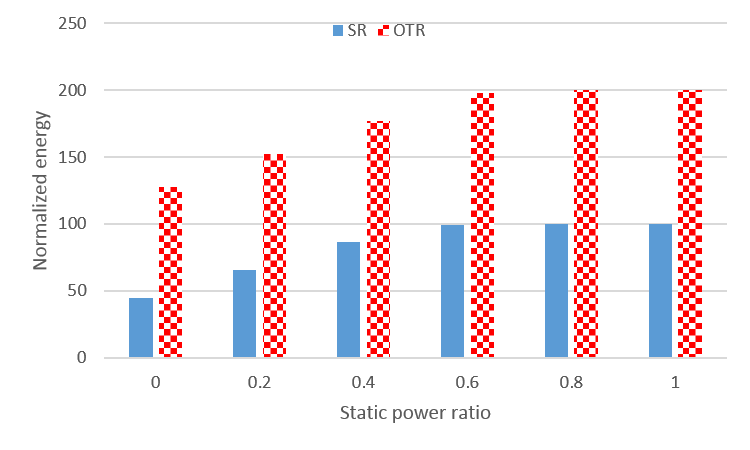
\includegraphics[width=0.45\textwidth]{figures/crash_power}
		}
		\subfigure[Sensitivity to laxity. $W=100$ hours, $\rho=0.3$, $MTBF=5$ years.]
		{
			\label{fig:crash_time}
			\includegraphics[width=0.45\textwidth]{figures/crash_time}
		}
        \subfigure[Sensitivity to workload. $\alpha=0.25$, $\rho=0.5$, $MTBF=5$ years.]
		{
			\label{fig:crash_w}
			\includegraphics[width=0.45\textwidth]{figures/crash_w}
		}
	\end{center}
	\caption{Comparison between Soft Replication and Traditional Process Replication for energy consumption under a single crash failure.}
	\label{fig:crash_eval}
\end{figure*}


